\chapter{Élements techniques}

\section{Parser}\label{sec:parser}

\section{Moteur de réécriture}

Le moteur de réécriture est chargé d'appliquer les règles de réécritures itérativement à partir de l'axiome pour obtenir le mot final.
Nous avons d'un côté l'axiome qui est le mot de départ et une liste de règles qui contient 2 données : le mot à remplacer et son remplaçant.
Le mot est réécrit en 2 temps :\\
\begin{itemize}
    \item On change toutes les occurrences du mot à remplacer par \$\{identifiant de la règle\}.
    \item On remplace toutes les occurrences de \$\{identifiant de la règle\} par la règle associée.
\end{itemize}
On répète cette opération n fois, pour obtenir le mot final.

\section{Moteur graphique}\label{src:interface3d}

Nous utilisons Java OpenGL pour afficher une fenêtre 3D, gl2 pour afficher les lignes de la grille, glu pour placer la caméra et GLUT pour afficher les cylindres.
Pour naviguer dans l'espace 3D, voir la section \ref{sec:nav_3d}

\begin{figure}[h!]
    \centering
    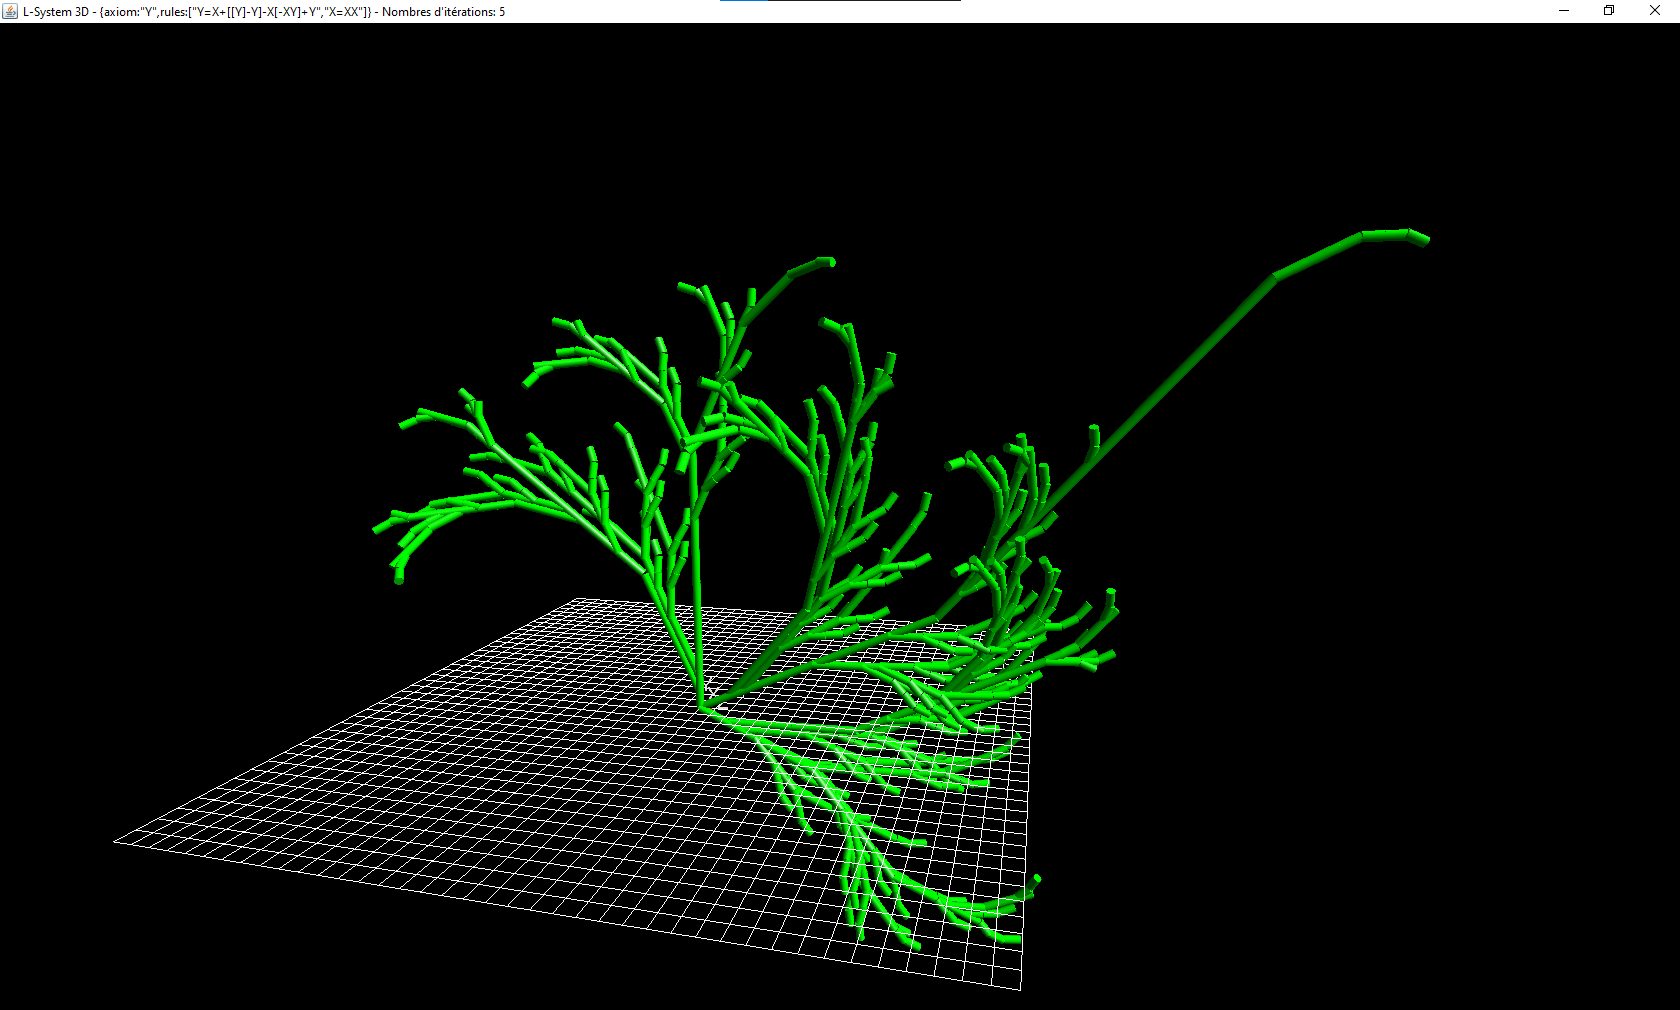
\includegraphics[width=0.8\linewidth]{pics/3dGUI.png}
    \caption{Fenêtre 3D}
    \label{fig:3d_frame}
\end{figure}

\clearpage

\section{Interface principale}\label{sec:menu}

\subsection{Composition de l'interface}

\paragraph{L'interface}
utilisateur de notre logiciel a été conçu grâce à la bibliothèque \Swing \ de \Java. Elle se compose de trois classes, une contenant la fenêtre principale \classe{MainFrame}, une autre permettant de créer des onglets, \classe{Tab} et une troisième classe gérant les événements, \classe{Listener}.

\subsection{Classes de l'interface}

\subsubsection{MainFrame}

\paragraph{La classe \classe{MainFrame}} est une classe héritant de la classe JFrame de \Swing. Elle permet de créer une fenêtre de base, de taille prédéfinie dans laquelle peuvent être placés des composants graphiques. Elle comprend aussi un bouton de fermeture qui, une fois cliqué, permet l'arrêt du programme.\\
Elle comporte aussi une instance de la classe JTabbedPane \label{jtpane}, un conteneur graphique donc le but est de disposer ses composants sous la forme d'onglets.

\subsubsection{Tab}

\paragraph{La classe \classe{Tab}} est une classe héritant de la classe JPanel de \Swing. JPanel est un composant de base dans lequel il est possible d'ajouter d'autres composants graphiques. Les intances de \classe{Tab} créées sont ensuite ajoutées par la classe \classe{MainFrame} à son composant de la classe JTabbedPane \ref{jtpane}.

\subsubsection{Listener}

\paragraph{La classe \classe{Listener}} est une classe implémentant certaines classes Listener de \Swing (\classe{ActionListener, KeyListener et MouseWheelListener}). Elle permet de capter toutes les actions effectuées par l'utilisateur et d'appeler les méthodes correspondantes des classes de l'interface. Elle permet ainsi de créer de nouveaux onglets (Nouvelles instances de Tab) mais aussi d'en fermer ou bien encore de lancer la génération du modèle.
\section{Pair ou un tuple a 2 entrées en java}
